\documentclass{beamer}

\usepackage{amsmath}
\usepackage{booktabs}
\usepackage{array}
\usepackage{tabularx}
\usepackage{graphicx}
\usepackage{adjustbox}
\usepackage{pgfpages}
\usetheme{sintef}

\ifdefined\shownotesoption
  \setbeameroption{show notes on second screen=right}
\else
  \setbeameroption{hide notes}
\fi

\usefonttheme[onlymath]{serif}
\titlebackground*{assets/background}

\newcommand{\ccc}{\mathrm{CCC}}
\newcommand{\topk}{top-$K$}
\newcommand{\smallgap}{\vspace{0.25em}}
\newcommand{\speechnote}[1]{\note{\scriptsize #1}}
\newcolumntype{Y}{>{\raggedright\arraybackslash}X}

\title{Evaluating the Quality of Explanations under a Cognitive Feature Budget}
\subtitle{Complexity-Calibrated Local Concordance for compact local explanations}
\course{Explainable and Trustworthy AI}
\author{Stefano Zizzi \and Michelangelo Ungolo \and Miriana Sette}
\IDnumber{}
\date{\today}

\AtBeginSection[]
{
    \begingroup
    \themecolor{main}
    \begin{frame}{Table of Contents}
        \tableofcontents[currentsection]
        \ifcase\value{section}
        \or \speechnote{We start from the metric, because this is the main contribution of the project.}
        \or \speechnote{Now that the metric is defined, Michelangelo will explain how we used it in the benchmark.}
        \or \speechnote{Now we move to the main results.}
        \or \speechnote{We now summarize the main takeaways.}
        \fi
    \end{frame}
    \endgroup
}

\begin{document}

\maketitle
\speechnote{
Good morning. We are Stefano Zizzi, Michelangelo Ungolo, and Miriana Sette.

Today we present our project, \textbf{Evaluating the Quality of Explanations under a Cognitive Feature Budget}.

The main idea is simple: in Explainable AI, we often evaluate whether a full explanation is faithful to the model. But in practice, users rarely see the full explanation. They usually see only a small number of features. So our question is: what happens to fidelity when the explanation is made short enough for a human to inspect?
}

\begin{frame}{Problem}
\framesubtitle{From full fidelity to displayed fidelity}
\begin{columns}[T,onlytextwidth]
\begin{column}{0.55\textwidth}
\begin{itemize}
  \item Local explainers often produce one contribution per feature.
  \item Standard fidelity can evaluate the complete additive reconstruction.
  \item Real interfaces usually display only a small number of features.
  \item A faithful full explanation can become misleading after truncation.
\end{itemize}
\end{column}
\begin{column}{0.39\textwidth}
\begin{colorblock}{maincolor}{Core question}
\centering
\small
How much model fidelity is preserved when only the \topk{} contributions are shown?
\end{colorblock}
\end{column}
\end{columns}
\speechnote{
Local explanation methods such as LIME, SHAP, and MAPLE usually assign one contribution to each input feature.

Many evaluation metrics check the complete explanation, meaning all feature contributions are included. However, real interfaces, dashboards, and reports normally display only the most important features.

This creates a gap between \textbf{full fidelity} and \textbf{displayed fidelity}. An explanation can reconstruct the model well when all features are used, but become much less faithful when only the top features are shown.

So the core question of the project is: \textbf{how much model fidelity is preserved when only the top-K contributions are displayed?}
}
\end{frame}

\section{Metric}

\begin{frame}{Contribution}
\framesubtitle{Compact faithfulness under a cognitive budget}
\begin{itemize}
  \item We introduce Complexity-Calibrated Local Concordance.
  \item CCC measures reconstruction error after enforcing a feature budget
        $K \in \{5,6,7,8,9\}$.
  \item Lower CCC means the displayed explanation better reconstructs the
        black-box probability.
  \item The metric complements full MSE, sufficiency, comprehensiveness, and
        random-$K$ baselines.
\end{itemize}
\speechnote{
To study this problem, we introduce \textbf{Complexity-Calibrated Local Concordance}, or \textbf{CCC}.

CCC is a budget-aware metric. Instead of asking whether the complete explanation reconstructs the model output, it asks whether the explanation still reconstructs the model output after keeping only K features.

We evaluate K from 5 to 9, following the idea of a limited cognitive budget. Lower CCC means lower reconstruction error, so the displayed explanation is more faithful to the black-box prediction.

The goal is not to replace existing metrics, but to complement them. CCC adds a specific view: fidelity under a human-sized feature budget.
}
\end{frame}

\begin{frame}{CCC Definition}
\framesubtitle{Budget-aware additive reconstruction}
\begin{columns}[T,onlytextwidth]
\begin{column}{0.54\textwidth}
\begin{align*}
g_K(x) &= w_0 + \sum_{i \in S_K(x)} \phi_i(x) \\
\ccc_K &=
\frac{1}{N}\sum_{j=1}^{N}
\left(f(x^{(j)}) - g_K(x^{(j)})\right)^2
\end{align*}
\end{column}
\begin{column}{0.42\textwidth}
\begin{itemize}
  \item $f(x)$ is the black-box positive-class probability.
  \item $w_0$ is the explainer intercept.
  \item $\phi_i(x)$ is the additive feature contribution.
  \item $S_K(x)$ keeps the $K$ largest absolute contributions.
\end{itemize}
\end{column}
\end{columns}
\speechnote{
Formally, for each instance we start from the black-box probability, called $f(x)$.

The explainer gives us an intercept $w_0$ and a vector of feature contributions, $\phi$.

We select $S_K$, the set of the K largest contributions in absolute value. Then we reconstruct the prediction using only those K terms: $g_K(x) = w_0$ plus the sum of the selected contributions.

CCC is the mean squared error between the black-box prediction and this truncated reconstruction.

So if CCC is low, the short explanation is still close to the model output. If CCC is high, the displayed explanation loses fidelity.
}
\end{frame}

\begin{frame}{Common Explainer Format}
\framesubtitle{Normalizing LIME, SHAP, and MAPLE}
\begin{table}
\centering
\small
\begin{tabularx}{\textwidth}{lY}
\toprule
Explainer & Additive contribution used by CCC \\
\midrule
SHAP & Shapley values are already additive contributions. \\
LIME & Local coefficients are multiplied by the interpretable representation:
$\phi_i = \beta_i z_i(x)$. \\
MAPLE & Local coefficients are multiplied by the feature value:
$\phi_i = \beta_i x_i$. \\
\bottomrule
\end{tabularx}
\end{table}
\smallgap
\begin{colorblock}[darkgray]{sintefgrey}{Assumption}
\small
All explainers are evaluated through the same form:
$g(x)=w_0+\sum_i \phi_i(x)$.
\end{colorblock}
\speechnote{
Since we compare different explainers, we first normalize them into the same additive format.

For SHAP, this is straightforward, because SHAP values are already additive contributions.

For LIME, the local coefficients are multiplied by the interpretable representation of the instance. This gives instance-level additive contributions.

For MAPLE, the coefficients are multiplied by the corresponding feature values.

The important assumption is that all methods are evaluated through the same structure: $g(x)=w_0+\sum_i \phi_i(x)$.

This makes the comparison consistent across LIME, SHAP, and MAPLE.
}
\end{frame}

\section{Benchmark}

\begin{frame}{Experimental Setup}
\framesubtitle{Datasets, models, explainers, and budgets}
\begin{columns}[T,onlytextwidth]
\begin{column}{0.48\textwidth}
\begin{block}{Datasets}
\begin{itemize}
  \item UCI Adult
  \item UCI Breast Cancer Wisconsin Diagnostic
\end{itemize}
\end{block}
\begin{block}{Classifiers}
\begin{itemize}
  \item XGBoost
  \item Neural network
\end{itemize}
\end{block}
\end{column}
\begin{column}{0.48\textwidth}
\begin{block}{Explainers}
\begin{itemize}
  \item LIME
  \item SHAP KernelExplainer
  \item MAPLE
\end{itemize}
\end{block}
\begin{block}{Evaluation}
\begin{itemize}
  \item $K=5,6,7,8,9$
  \item Seeds 42, 123, 2026
\end{itemize}
\end{block}
\end{column}
\end{columns}
\speechnote{
The benchmark uses two tabular datasets: UCI Adult and UCI Breast Cancer Wisconsin Diagnostic.

We test two black-box classifiers: XGBoost and a neural network.

For explanations, we compare three local methods: LIME, SHAP KernelExplainer, and MAPLE.

For each dataset, model, and explainer combination, we compute CCC for K equal to 5, 6, 7, 8, and 9. We also repeat the experiments over three random seeds: 42, 123, and 2026.

This gives us a controlled setting where we can observe how compact fidelity changes as the feature budget increases.
}
\end{frame}

\begin{frame}{Benchmark Pipeline}
\framesubtitle{Reproducible local explanation evaluation}
\begin{enumerate}
  \item Load and scale the dataset.
  \item Train each configured black-box classifier.
  \item Generate local explanations for each model and explainer pair.
  \item Convert explanations into additive contributions.
  \item Compute CCC, full MSE, random-$K$, sufficiency, and comprehensiveness.
\end{enumerate}
\smallgap
\begin{colorblock}{maincolor}{Implementation}
\small
The orchestration is implemented in \texttt{core/test\_framework.py}; metrics are implemented in \texttt{core/metrics.py}.
\end{colorblock}
\speechnote{
The benchmark pipeline is reproducible.

First, we load and scale the dataset. Then we train each black-box classifier.

After that, we generate local explanations for each model and explainer pair. These explanations are converted into the common additive format described before.

Finally, we compute several metrics: CCC, full MSE, random-K MSE, sufficiency, and comprehensiveness.

The orchestration is implemented in \texttt{core/test\_framework.py}, while the metric definitions are implemented in \texttt{core/metrics.py}.
}
\end{frame}

\begin{frame}{Model Accuracy}
\framesubtitle{Accuracy alone does not select the best explainer}
\begin{table}
\centering
\begin{tabular}{llr}
\toprule
Dataset & Model & Mean accuracy \\
\midrule
Adult & XGBoost & 0.874 \\
Adult & Neural network & 0.823 \\
Breast Cancer & XGBoost & 0.968 \\
Breast Cancer & Neural network & 0.977 \\
\bottomrule
\end{tabular}
\end{table}
\smallgap
\begin{itemize}
  \item High model accuracy does not imply compact explanations.
  \item CCC measures the displayed explanation, not the classifier alone.
\end{itemize}
\speechnote{
This slide shows the mean model accuracy across the three seeds.

The classifiers perform well overall. For example, XGBoost reaches about 0.874 accuracy on Adult, and the neural network reaches about 0.977 on Breast Cancer.

But the key point is that accuracy alone does not tell us which explainer is better.

A model can be accurate and still difficult to explain compactly. CCC measures the quality of the displayed explanation, not just the classifier performance.
}
\end{frame}

\section{Results}

\begin{frame}{CCC Curves}
\framesubtitle{Lower curves mean more faithful compact explanations}
\centering
\vspace{-0.8em}
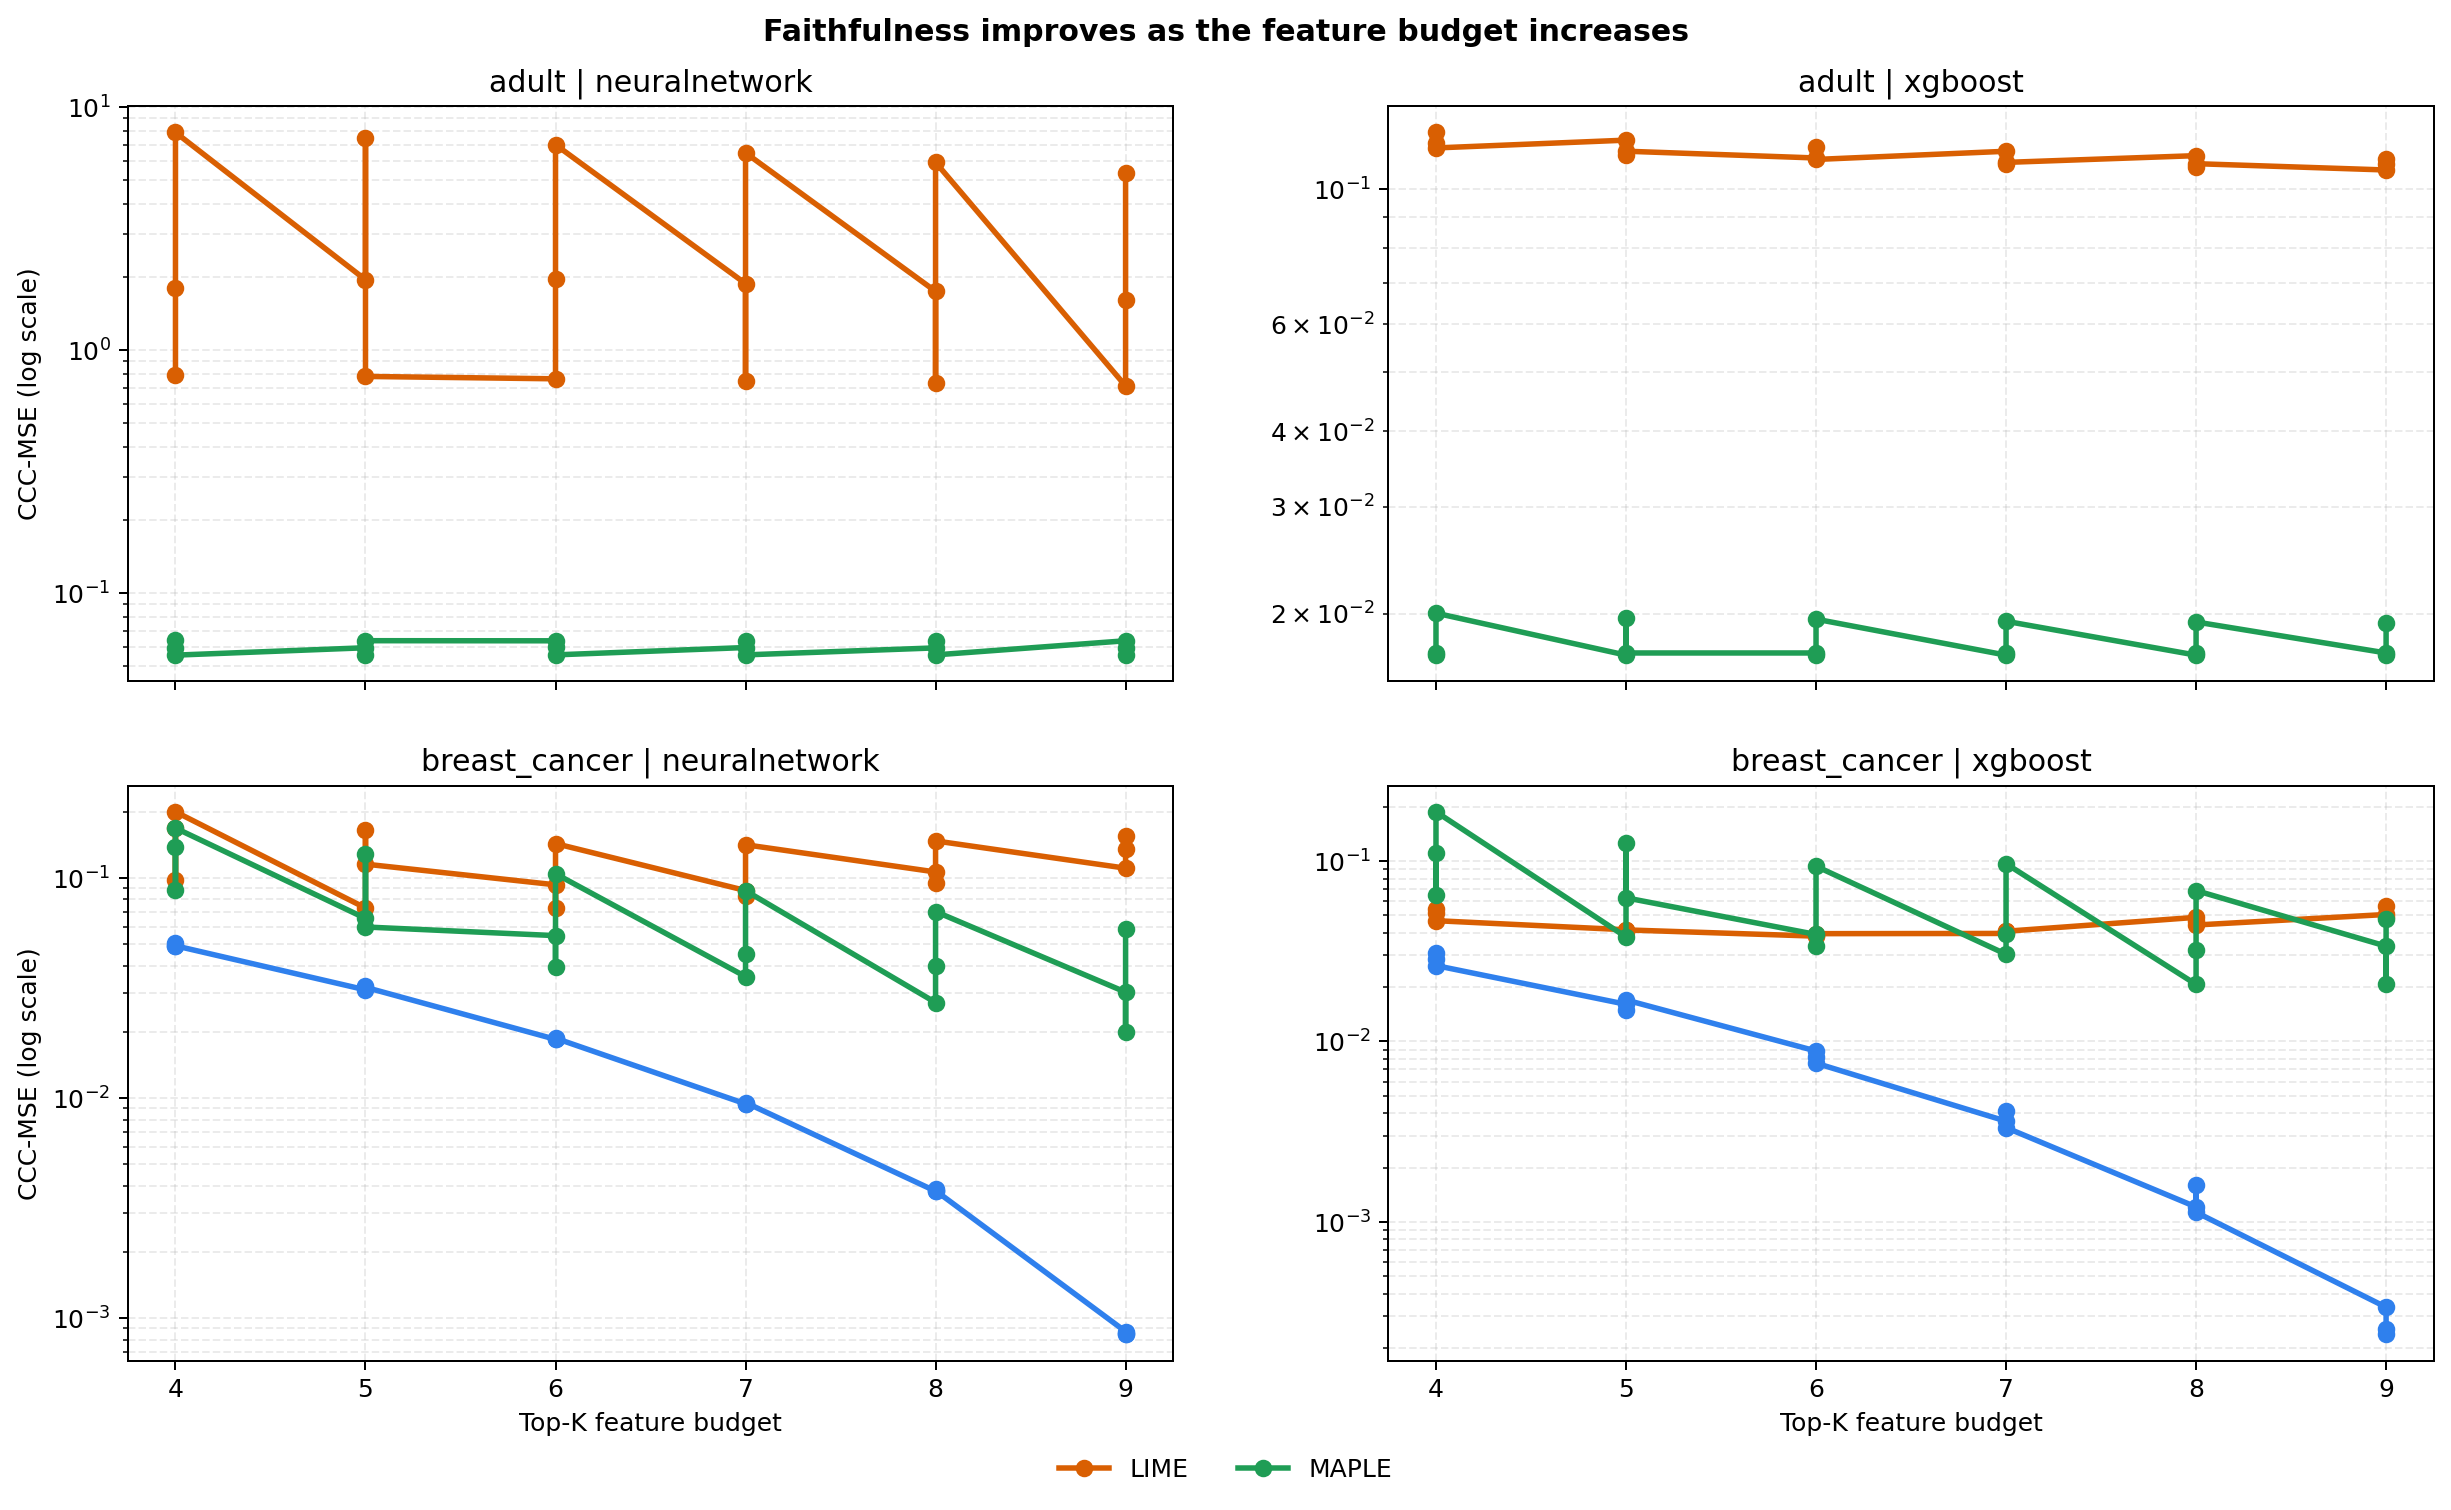
\includegraphics[width=1.08\textwidth,height=0.88\textheight,keepaspectratio]{../../results/figures/latest/ccc_mse_by_k.png}
\speechnote{
This figure shows CCC as K increases.

The lower the curve, the more faithful the compact explanation is. In general, SHAP has the lowest curves, especially as K increases.

This is expected because SHAP has a strong additive reconstruction property. But the important observation is that CCC is not always zero at small K. Even if the full explanation is faithful, the compact version can still lose information.

MAPLE is usually intermediate. In some cases it improves with K, while in others it stays almost flat.

LIME is the most unstable, and in some Breast Cancer settings the error does not decrease monotonically.
}
\end{frame}

\begin{frame}{Representative CCC Values}
\framesubtitle{Lower is better}
\centering
\scriptsize
\begin{adjustbox}{max width=\textwidth}
\begin{tabular}{llrrrrr}
\toprule
Dataset/model & Explainer & $K=5$ & $K=6$ & $K=7$ & $K=8$ & $K=9$ \\
\midrule
Adult/NN & SHAP   & 0.0072 & 0.0040 & 0.0020 & 0.0008 & 0.0002 \\
Adult/NN & MAPLE  & 0.0574 & 0.0574 & 0.0574 & 0.0574 & 0.0574 \\
Adult/NN & LIME   & 3.8262 & 3.6462 & 3.4261 & 3.1941 & 2.9571 \\
Adult/XGB & SHAP  & 0.0014 & 0.0007 & 0.0003 & 0.0001 & 0.0000 \\
Adult/XGB & MAPLE & 0.0181 & 0.0180 & 0.0179 & 0.0179 & 0.0179 \\
Adult/XGB & LIME  & 0.1168 & 0.1139 & 0.1119 & 0.1104 & 0.1095 \\
Breast/NN & SHAP  & 0.0318 & 0.0183 & 0.0094 & 0.0037 & 0.0009 \\
Breast/NN & MAPLE & 0.0847 & 0.0670 & 0.0565 & 0.0462 & 0.0365 \\
Breast/NN & LIME  & 0.1269 & 0.1111 & 0.1084 & 0.1220 & 0.1368 \\
Breast/XGB & SHAP & 0.0160 & 0.0082 & 0.0037 & 0.0014 & 0.0003 \\
Breast/XGB & MAPLE & 0.0755 & 0.0556 & 0.0555 & 0.0405 & 0.0341 \\
Breast/XGB & LIME & 0.0398 & 0.0370 & 0.0412 & 0.0470 & 0.0521 \\
\bottomrule
\end{tabular}
\end{adjustbox}
\speechnote{
This table gives representative aggregate CCC values.

On Adult with the neural network, SHAP decreases from about 0.007 at K equal to 5 to almost zero at K equal to 9.

MAPLE is almost flat in the Adult cases, meaning that increasing K does not recover much additional reconstruction signal.

LIME on Adult with the neural network is much worse, with CCC above 3 even at K equal to 9.

On Breast Cancer, SHAP again improves strongly as K increases. MAPLE improves more gradually. LIME is interesting because it can improve at first and then get worse.
}
\end{frame}

\begin{frame}{Explainer Patterns}
\framesubtitle{What the CCC curves reveal}
\begin{columns}[T,onlytextwidth]
\begin{column}{0.31\textwidth}
\begin{block}{SHAP}
\small
Lowest CCC overall. Error decreases quickly as $K$ grows, but small budgets can still lose fidelity.
\end{block}
\end{column}
\begin{column}{0.31\textwidth}
\begin{block}{MAPLE}
\small
Intermediate behavior. Some settings improve with $K$; Adult is almost flat, suggesting weak top-$K$ concentration.
\end{block}
\end{column}
\begin{column}{0.31\textwidth}
\begin{block}{LIME}
\small
Most unstable. On Breast Cancer, CCC is non-monotonic because local surrogate weights do not guarantee additive accuracy.
\end{block}
\end{column}
\end{columns}
\speechnote{
The results show three main patterns.

First, SHAP gives the best compact reconstructions overall. Its error decreases quickly as more features are included.

Second, MAPLE behaves like an intermediate baseline. It can recover some signal, but its top-ranked features are not always strongly concentrated.

Third, LIME is the most sensitive method. Its local surrogate does not guarantee that the selected additive terms reconstruct the black-box probability well.

This is exactly the type of behavior CCC is designed to expose.
}
\end{frame}

\begin{frame}{Why LIME Can Be Non-Monotonic}
\framesubtitle{Adding features can increase squared reconstruction error}
\begin{itemize}
  \item LIME refits a local sparse surrogate and does not enforce local accuracy.
  \item Feature selection is not guaranteed to be nested across values of $K$.
  \item Breast Cancer features are highly correlated, so added terms can change
        the reconstruction direction.
  \item Ranking by absolute contribution can add terms whose signs increase
        $|f(x)-g_K(x)|$.
\end{itemize}
\smallgap
\begin{colorblock}{sintefyellow}{Example}
\small
Breast/NN LIME improves from $K=5$ to $K=7$ but worsens at $K=8$ and $K=9$:
0.1269, 0.1111, 0.1084, 0.1220, 0.1368.
\end{colorblock}
\speechnote{
LIME can be non-monotonic because adding one more feature does not necessarily reduce the squared reconstruction error.

There are several reasons for this. LIME fits a local sparse surrogate and does not enforce local accuracy. The selected feature set is not guaranteed to be nested across different K values. Also, Breast Cancer features are highly correlated, so added terms can interact with the reconstruction direction.

In the example shown here, Breast Cancer with the neural network improves from K equal to 5 to K equal to 7, but then worsens at K equal to 8 and 9.

So this is not necessarily a bug. It shows that LIME's local weights can be unstable under a compact additive reconstruction metric.

I will now pass to Miriana, who will compare CCC with the other metrics and conclude the presentation.
}
\end{frame}

\begin{frame}{CCC Versus Full MSE}
\framesubtitle{Full fidelity is not compact fidelity}
\begin{columns}[T,onlytextwidth]
\begin{column}{0.48\textwidth}
\begin{table}
\centering
\scriptsize
\begin{adjustbox}{max width=\textwidth}
\begin{tabular}{lrrrrr}
\toprule
$K$ & 5 & 6 & 7 & 8 & 9 \\
\midrule
full MSE & 0.0 & 0.0 & 0.0 & 0.0 & 0.0 \\
CCC & 0.0160 & 0.0082 & 0.0037 & 0.0014 & 0.0003 \\
\bottomrule
\end{tabular}
\end{adjustbox}
\end{table}
\end{column}
\begin{column}{0.47\textwidth}
\begin{itemize}
  \item Example: SHAP on Breast Cancer/XGBoost.
  \item Full additive reconstruction is exact.
  \item The displayed \topk{} explanation still has measurable error.
\end{itemize}
\end{column}
\end{columns}
\speechnote{
This slide shows why CCC adds information beyond full MSE.

The example is SHAP on Breast Cancer with XGBoost. The full MSE is zero for every K, because the complete SHAP reconstruction is exact.

However, CCC is not zero when we keep only the top features. At K equal to 5, CCC is 0.0160, and it decreases as K increases.

This means that full fidelity and compact fidelity are different concepts. Full MSE says the complete explanation is faithful. CCC says how much fidelity remains when the explanation is shortened.
}
\end{frame}

\begin{frame}{Top-$K$ Versus Random-$K$}
\framesubtitle{The ranking should beat arbitrary feature subsets}
\centering
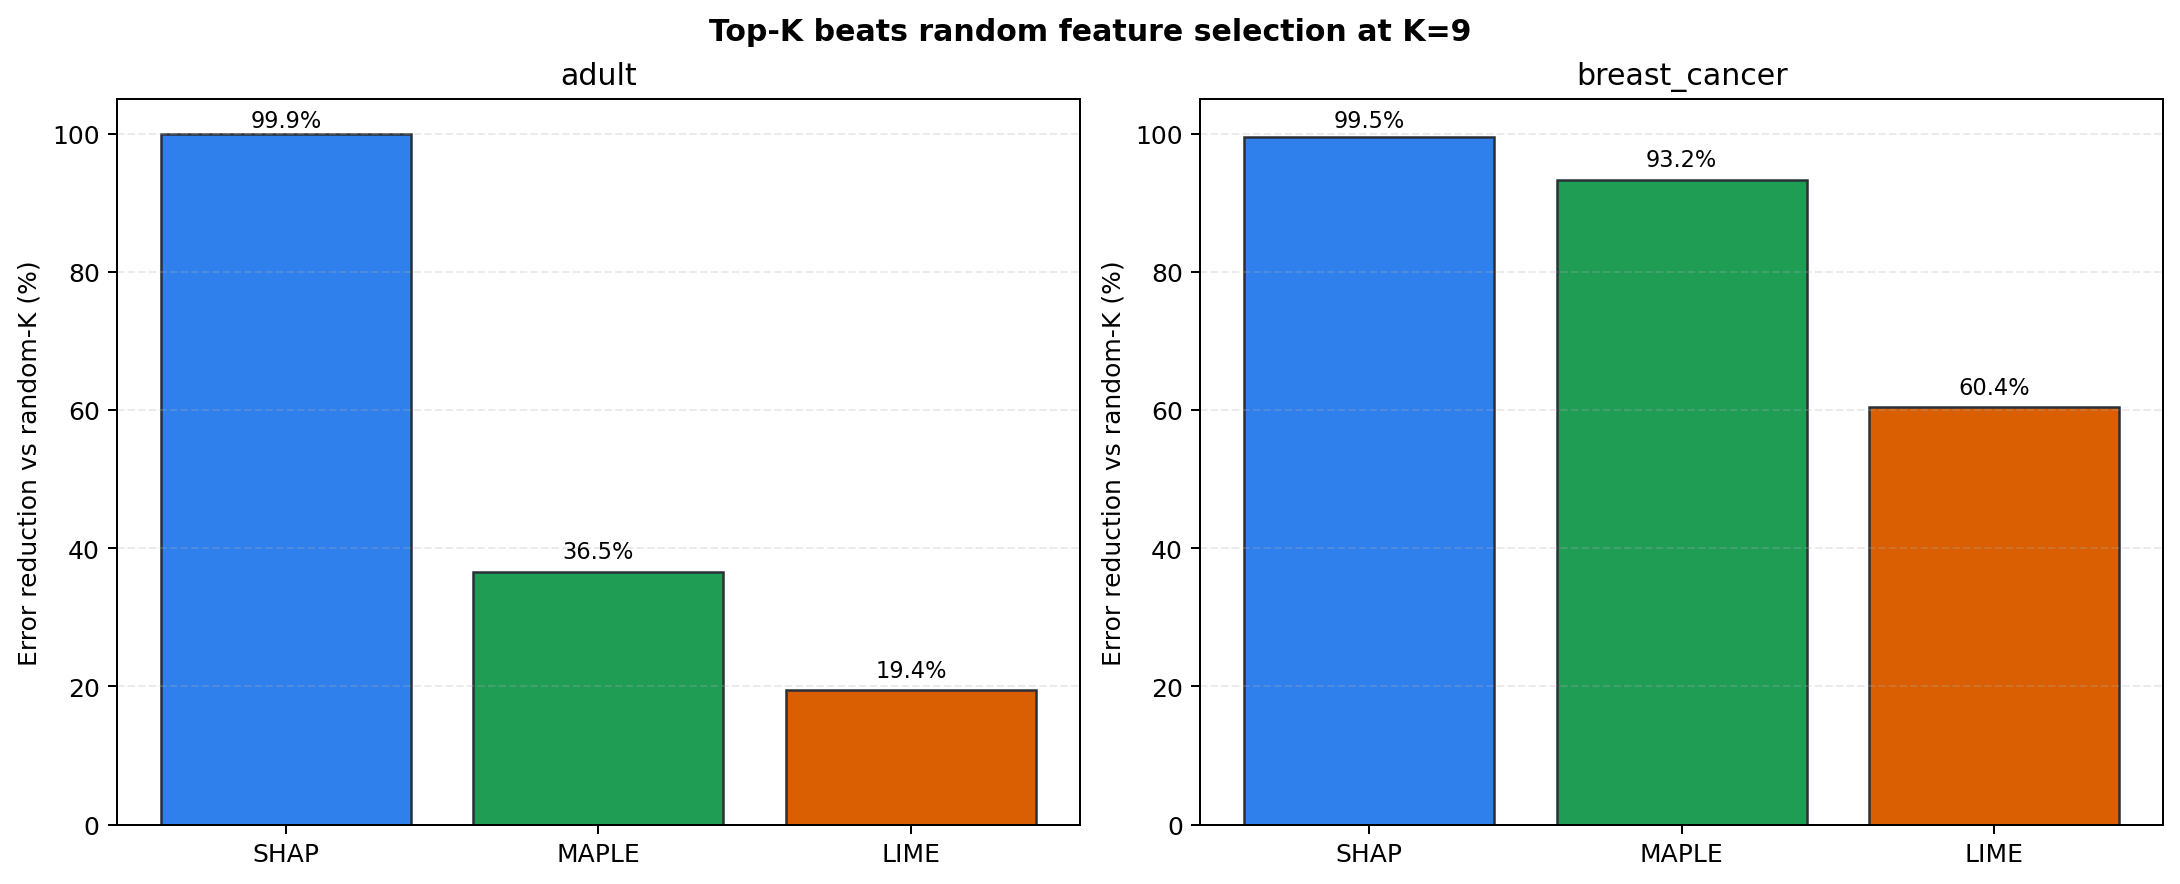
\includegraphics[width=0.9\textwidth,height=0.67\textheight,keepaspectratio]{../../results/figures/latest/top_k_vs_random_k_k9.png}
\speechnote{
The random-K baseline is an internal sanity check.

If the explainer ranking is meaningful, the top-K features should reconstruct the prediction better than a random subset of K features.

In most settings, this is exactly what we observe. Top-K CCC is much lower than random-K MSE, especially for SHAP.

When the gap is smaller, it suggests that the explainer's feature ranking is less informative.
}
\end{frame}

\begin{frame}{Metric Comparison}
\framesubtitle{CCC answers a different evaluation question}
\scriptsize
\begin{tabularx}{\textwidth}{lY}
\toprule
Metric & Relation to CCC \\
\midrule
Full MSE & Evaluates all-feature reconstruction; CCC evaluates after top-$K$ truncation. \\
Sufficiency & Keeps selected input features under a masking baseline; CCC evaluates additive concordance directly. \\
Comprehensiveness & Measures prediction change after removing selected features; CCC asks whether displayed additive terms reconstruct $f(x)$. \\
Infidelity or sensitivity & Measures stability under input perturbations; CCC adds an explicit cognitive feature budget. \\
Conciseness & Measures explanation size alone; CCC combines compactness with predictive faithfulness. \\
\bottomrule
\end{tabularx}
\speechnote{
CCC answers a different question from the other metrics.

Full MSE evaluates the complete additive reconstruction. CCC evaluates the reconstruction after top-K truncation.

Sufficiency and comprehensiveness are perturbation metrics: they modify the input and observe how the model prediction changes.

CCC does not perturb the input. Instead, it directly asks whether the displayed additive terms reconstruct the black-box probability.

So CCC is especially useful when the explanation is actually shown to a user as a short list of feature contributions.
}
\end{frame}

\section{Takeaways}

\begin{frame}{What CCC Adds}
\framesubtitle{A practical lens for human-sized explanations}
\begin{itemize}
  \item CCC separates model accuracy, full explanation fidelity, and compact explanation fidelity.
  \item It exposes how quickly the top-ranked features recover the model prediction.
  \item It can be summarized as a curve, an area under the CCC curve, or a minimum faithful $K$.
  \item It is useful as an offline benchmark and as a runtime warning for deployed explanation tools.
\end{itemize}
\speechnote{
CCC separates three ideas that are often mixed together: model accuracy, full explanation fidelity, and compact explanation fidelity.

It also gives a full curve across different values of K. This curve tells us how quickly the top-ranked features recover the model prediction.

In practice, CCC could be summarized using the area under the CCC curve, or by finding the smallest K that reaches an acceptable error threshold.

This makes CCC useful both as an offline benchmark metric and as a possible runtime warning in deployed explanation tools.
}
\end{frame}

\begin{frame}{Limitations and Extensions}
\framesubtitle{Where the metric should be pushed next}
\begin{columns}[T,onlytextwidth]
\begin{column}{0.48\textwidth}
\begin{block}{Limitations}
\begin{itemize}
  \item Designed for additive explanations.
  \item Depends on probability scale and calibration.
  \item Fixed $K$ is only a proxy for cognitive complexity.
  \item Current benchmark covers two datasets and two model families.
\end{itemize}
\end{block}
\end{column}
\begin{column}{0.48\textwidth}
\begin{block}{Extensions}
\begin{itemize}
  \item Add datasets and black-box models.
  \item Choose the smallest $K$ below an error threshold.
  \item Integrate CCC into explanation dashboards.
\end{itemize}
\end{block}
\end{column}
\end{columns}
\speechnote{
There are also limitations.

CCC is designed for additive explanations, so it does not directly apply to rule lists, counterfactual explanations, or prototypes.

It also depends on the scale and calibration of predicted probabilities, so raw CCC values should be interpreted carefully when moving across datasets.

Another limitation is that a fixed K is only a proxy for cognitive complexity. For example, one-hot encoded features may not correspond to human-level concepts.

As future work, the benchmark could be extended to more datasets, more model families, and adaptive values of K.
}
\end{frame}

\begin{frame}{Conclusion}
\framesubtitle{Compact faithfulness is a distinct target}
\begin{itemize}
  \item Full explanation fidelity does not guarantee faithful displayed explanations.
  \item CCC evaluates the fidelity of the explanation that a user actually sees.
  \item In this benchmark, SHAP gives the strongest compact reconstructions, MAPLE is intermediate, and LIME is more sensitive to $K$ and local instability.
  \item Explainer selection should combine CCC with perturbation metrics when practical decisions depend on both reconstruction and input-masking behavior.
\end{itemize}
\speechnote{
The main conclusion is that compact faithfulness is a distinct evaluation target.

An explanation can be faithful when all features are included, but less faithful when only the displayed top-K features are used.

CCC measures exactly this displayed-explanation fidelity.

In our benchmark, SHAP gives the strongest compact reconstructions, MAPLE is intermediate, and LIME is more sensitive to K and local instability.

More generally, explainer selection should not depend on a single metric. CCC should be used together with perturbation metrics when practical decisions depend on both additive reconstruction and input-masking behavior.
}
\end{frame}

\begingroup
\themecolor{main}
\begin{frame}[c]
  \centering
  \begin{minipage}{\textwidth}
    \usebeamercolor[fg]{normal text}
    \centering
    \Huge \inserttitle
    \vspace{5mm}

    \Large \textsl{Thank you for listening!}\\[2mm]
    \Large \textsl{Any questions?}
  \end{minipage}
\speechnote{
Thank you for listening. We are happy to answer any questions.
}
\end{frame}
\endgroup

\end{document}
